\section{Simulador Rayos-X}
\label{result:xray}

\begin{figure}[h]
\centering
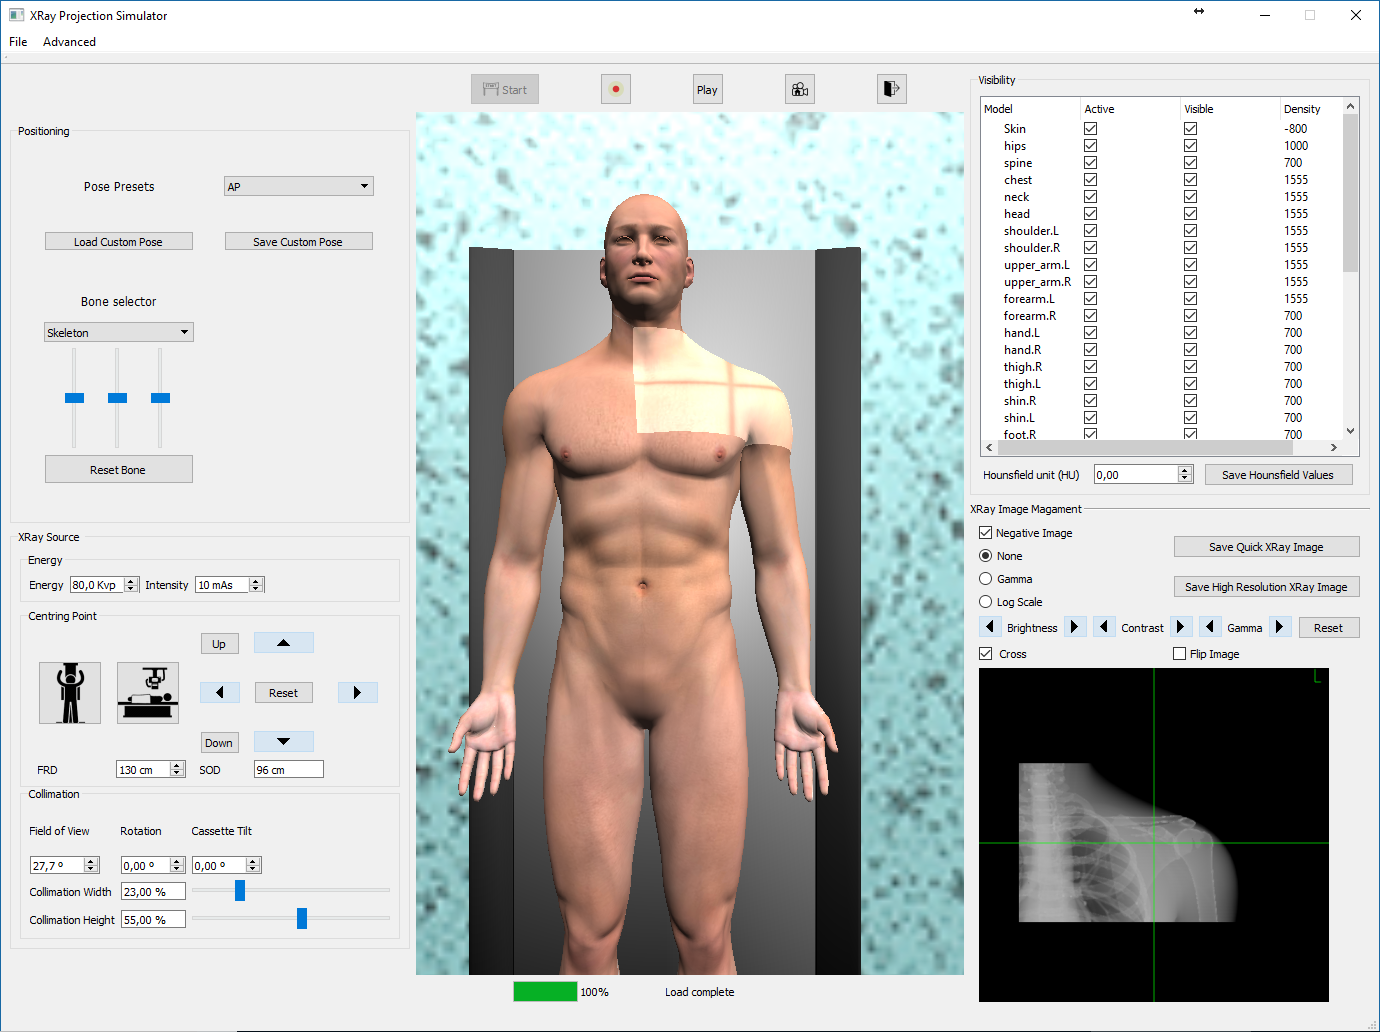
\includegraphics[width=0.95\linewidth]{IMG/simui.png}
\caption{\label{fig:simui} Interfaz de usuario del simulador de radiología diagnóstica. }
\end{figure}

En la figura \ref{fig:simui} se puede observar como es la interfaz de usuario del simulador de radiología diagnóstica. En esta imagen se puede observar todas las funcionalidades del simulador. 
En la zona central, se encuentra la vista de la escena 3D. En esta ventana, se podrá observar el modelo virtual cargado para la ocasión situado en una sala de radiología virtual. El usuario podrá utilizar el ratón para mover la perspectiva de la cámara y hacerse una idea de la escena virtual.
En la esquina superior izquierda se sitúa el módulo de posicionamiento del modelo virtual. En esta división, el usuario puede seleccionar posturas previamente guardadas o almacenar nuevas posiciones. Además, puede seleccionar de manera individual cada articulación que disponga el modelo virtual. 

En la esquina inferior izquierda, se puede observar todos los parámetros relacionados con la configuración del emisor de rayos X con el objetivo de conseguir una imagen radiográfica de calidad.
Por otra parte, en la esquina superior derecha se encuentra una lista de los tejidos del paciente virtual que están disponibles. En esta lista, se puede esconder los tejidos bajo demanda o se puede cambiar sus propiedades químicas. Esta funcionalidad permite al usuario comprobar multitud de variaciones del modelo virtual cargado.

Por último, en la esquina inferior derecha se puede observar la imagen de rayos X resultante de la posición del emisor en relación con el modelo virtual. En esta imagen se podrá apreciar la configuración de la colimación o de los distintos parámetros que definen un emisor de rayos X. Además, la imagen resultante puede ser modificada en cuanto a brillo, contraste, o filtros de imágenes. Esto ayuda al usuario a interpretar y entender la imagen al ocultar o resaltar detalles de la anatomía.

En cuanto al rendimiento de la aplicación, ambos algoritmos (posicionador de pacientes virtuales y la librería de simulación de rayos X) se ejecutan interactivamente. En el peor de los casos, el modelo de \emph{ZygoteBody}$^{TM}$ y su malla de tetraedros se componen de 1.5 millones de vértices y 2.5 millones de tetraedros. El simulador es capaz de mantenerse por encima de las 30 imágenes por segundo en un computador con las siguientes características: procesador \emph{Intel®i7-3770 @ 3.7GHz} con una tarjeta gráfica \emph{NVIDIA® Quadro K5000} y \emph{16 GB de \ac{RAM}}. 
El mayor consumo de tiempo viene dado por el proceso previo del algoritmo propuesto (ver sección \ref{posing:result}) y la complejidad del modelo virtual, que en el caso de \emph{ZygoteBody}$^{TM}$ toma menos de 7 minutos.

Los modelos anatómicos disponibles en el capítulo del posicionador de pacientes virtuales (sec. \ref{posing:result}) se han utilizado como modelos de entrada en el simulador. 

A continuación, se procederá a mostrar algunos resultados y comparaciones entre la aplicación desarrollada y un libro tradicional de proyecciones radiológicas.

\todo{Obviamente, hacer imagen}
Como se puede observar en la figura \ref{fig:xraycomp}, se han seleccionado unas imágenes de proyecciones radiológicas procedentes del libro \cite{carver2012medical} y se ha procedido a replicar la misma posición en la herramienta. La ventaja de usar la aplicación es que se pueden obtener más imágenes de la misma anatomía o proyección que permitirá a profesores y estudiantes practicar de manera más extensa. 


\begin{figure}[tb]
\centering
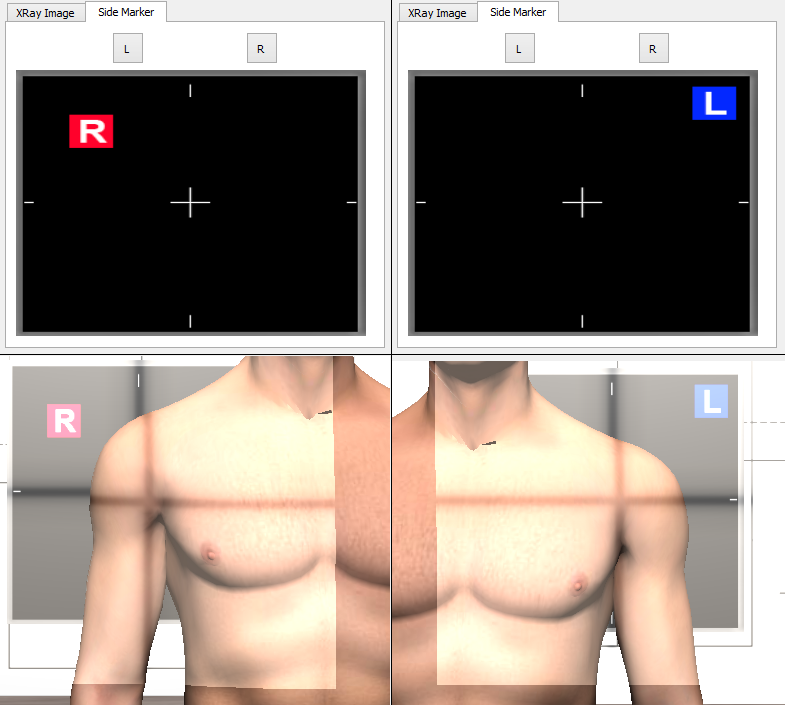
\includegraphics[width=0.5\linewidth]{IMG/side.png}
\caption{\label{fig:xraycomp} Comparativa entre una imagen del libro\cite{carver2012medical} y la imagen resultante de la herramienta. }
\end{figure}

Otra muestra de las ventajas del simulador frente a los materiales educativos tradicionales se puede observar en la figura \ref{fig:resultdisease}. En esta ocasión, es posible generar variaciones anatómicas del mismo modelo. Con ello se pueden enseñar como podría verse una enfermedad y ayudar a la interpretación la imagen. Cambiando unos pocos parámetros, el simulador permite cambiar entre un tejido sano o enfermo. Incluso puede ser interesante que los estudiantes puedan observar como objetos extraños se pueden distinguir cuando se encuentran dentro de la anatomía del paciente. 

\begin{figure}[tb]
\centering
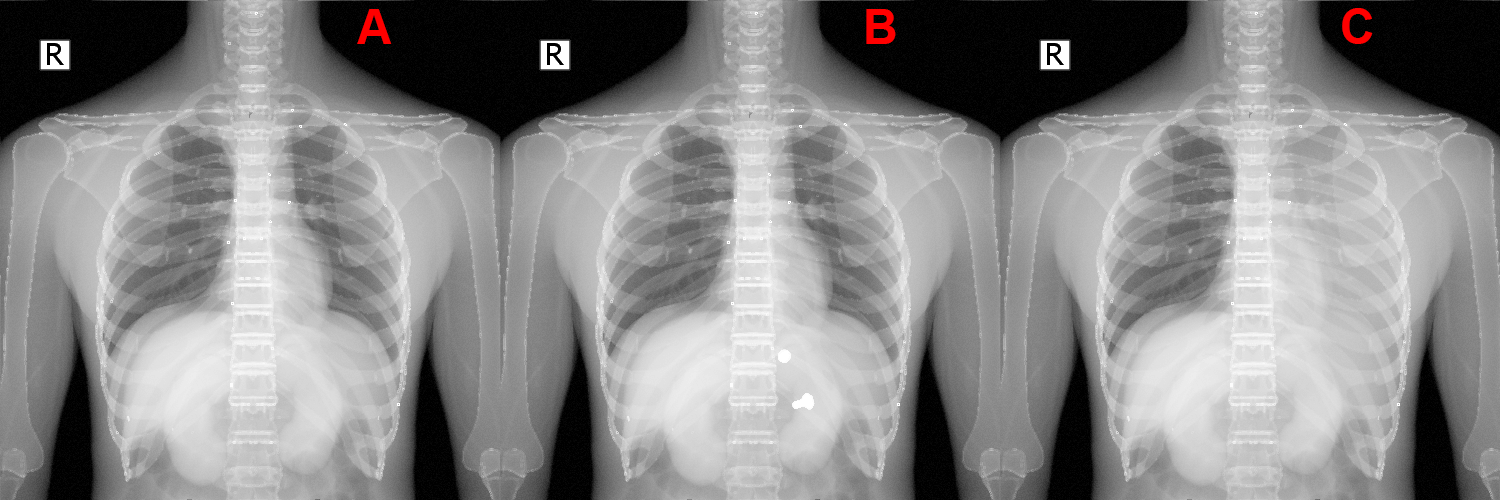
\includegraphics[width=0.5\linewidth]{IMG/disease.png}
\caption{\label{fig:resultdisease}Usuarios pueden probar diferentes casos. A: Anatomía normal. B: Objetos extraños en el estómago. C: Pulmón izquierdo colapsado. }
\end{figure}

\subsection{Discusión}

Los resultados del simulador muestran una herramienta educativa muy completa que puede ser usada como material complementario para los estudiantes de radiología. La aplicación proporciona un entorno seguro e interactivo para comprobar todo tipo de situaciones. El posicionador de pacientes virtuales permite una interacción en tiempo real con la posibilidad de generar una cantidad de variaciones anatómicas superior a los métodos clásicos como pueden ser los libros o archivos de casos.

Esta herramienta también demuestra la versatilidad del algoritmo presentado en esta tesis, ya que puede ser incorporado en cualquier simulador que necesite deformaciones plausibles en tiempos interactivos, permitiendo incluso que sea el usuario quien decida la posición final.

Aunque la aplicación se ha diseñado para satisfacer las necesidades de los radiólogos, esta presenta ciertas limitaciones respecto al procedimiento de diagnóstico por imagen. Existen cuestiones relacionadas con la preparación del paciente para el procedimiento que no pueden ser cubiertas por el simulador, entre ellas las siguientes:

\begin{itemize}
    \item Se recomienda utilizar un lenguaje apropiado y efectivo en la comunicación con los pacientes que no es posible recoger por el simulador.
    \item No se representa la necesidad de indicar al paciente acerca de quitarse prendas u objetos que afecten al área de examen.
    \item No se practican las recomendaciones en cuanto al uso de protectores de plomo para pacientes y profesionales.
    \item Otras comprobaciones que implican condiciones médicas o protocolarias como embarazo, identificación del paciente, etc...
\end{itemize}
